\title{BT5110 Data Management and Warehousing}

\subtitle{Tutorial 4: Entity-relationship Modelling}

\author{Mark Meng Huasong}

\institute[National University of Singapore] % (optional, but mostly needed)
{
	School of Computing\\
	National University of Singapore
}

\titlegraphic{
	
\includegraphics[width=2cm]{nus-logo}
}

\date{13 - 17 Sep, 2021}

\begin{frame}
	\titlepage
	\begin{tcolorbox}
		\begin{center}
			{\scriptsize \textcolor{red}{All the materials within presentation slides are protected by copyrights.\\
					It is forbidden by NUS to upload these materials to the Internet.}}
		\end{center}
	\end{tcolorbox}
\end{frame}

\begin{frame}[fragile]{Quick Recap: End of Last Tutorial}
	What we have done in the last week:\\\vspace{5pt}
	(1) Write simple queries with aggregation;\\
	(2) Write nested queries;\\
	(3) Make use of double negation and left outer joining to achieve complex queries. \\\vspace{5pt}
	\textcolor{brown}{(This tutorial does not use the existing book loan database)}
\end{frame}

\section*{Question 1 Entity-relationship Design}

\begin{frame}[fragile]{Question 1 (a-b)}
(a) Identify the entity sets. Justify your choice by quoting the sentences in the text that support it.\\ \vspace{5pt}
\textbf{Solution}: There are three entity sets: \texttt{member}, \texttt{bottle} and \texttt{wine}.\\ \vspace{10pt}

(b) Identify the relationship sets and the entity sets that they associate. Justify your choice by quoting the sentences in the text that support it.\\ \vspace{5pt}
\textbf{Solution}: There are two relationship sets: \texttt{taste} and \texttt{contain}. The relationship set \texttt{taste} links the entity set \texttt{member} with the entity set \texttt{bottle}. The relationship set \texttt{contain} links the entity set \texttt{wine} with the entity set \texttt{bottle}.
\end{frame}

\begin{frame}[fragile]{Question 1 (a-b) Cont.}
(c) For each entity set and relationship set identify its attributes. Justify your choice by quoting the sentences in the text that support it.\\ \vspace{5pt}
\textbf{Solution}: The relationship set \texttt{taste} has two attributes: date and rating. The relationship set \texttt{contain} has \textbf{\textit{no}} attribute. \\ \vspace{10pt}
	
(d) For each entity set, identify its keys.\\ \vspace{5pt}
\textbf{Solution}: For the entity set \texttt{member}, there are three attributes: name, address and card number. The card number is the primary key.\\\vspace{3pt}
For the entity set \texttt{wine}, there are 7 attributes. Three attributes appellation, name and vintage are (composite) keys; four remaining attributes are country of origin, degree of alcohol, certification and bottled details.\\\vspace{3pt}
For the entity set \texttt{bottle}, there are \textcolor{red}{\textbf{5}} attributes, including in cellar, bottle number and three foreign keys to identify a wine instance. The bottle number is the primary key, and the primary key(s) of the entity set \texttt{wine} is/are the referencing foreign keys. (The Boolean attribute can be derived by in cellar, therefore is not necessary.)
\end{frame}

\begin{frame}[fragile]{\textcolor{red}{Temp. slide}}

How may attributes for the entity set ``bottle''?
\begin{figure}
\begin{columns}
	\column{0.31\textwidth}
	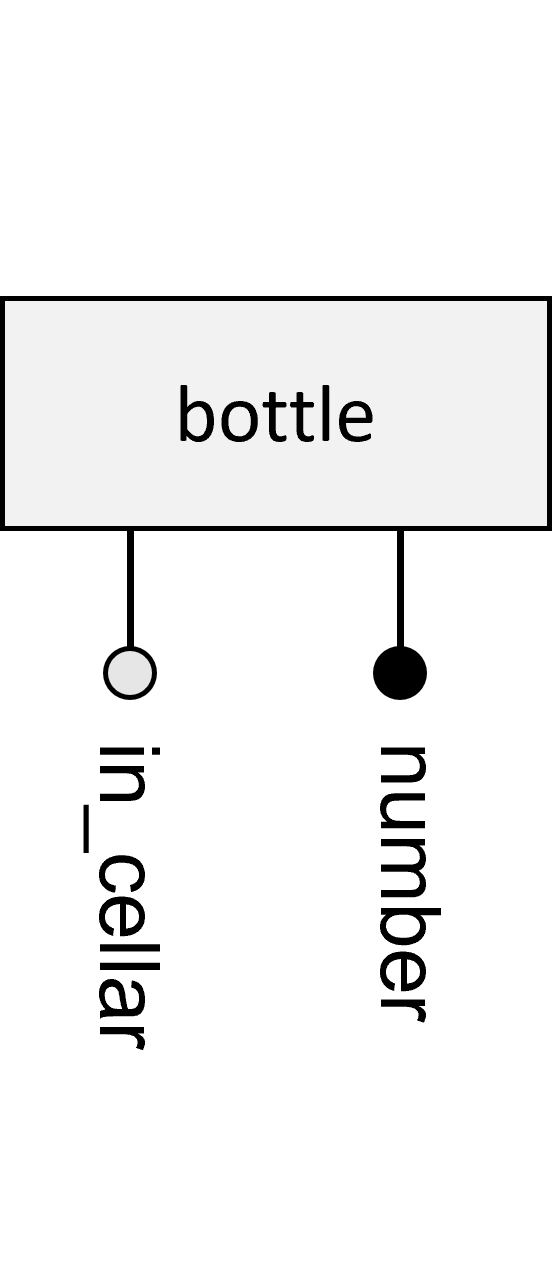
\includegraphics[width=1\textwidth]{t4/images/bottle_entity.png}
	\column{0.31\textwidth}
	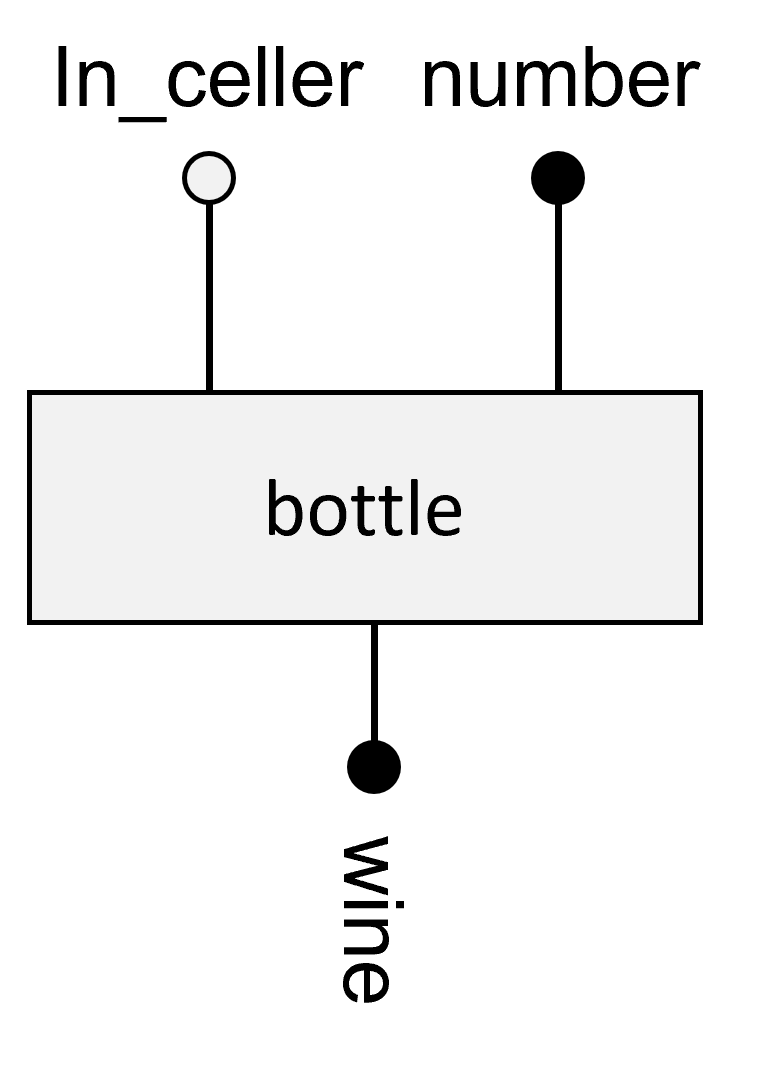
\includegraphics[width=1\textwidth]{t4/images/bottle_entity_1fk.png}
	\column{0.31\textwidth}
	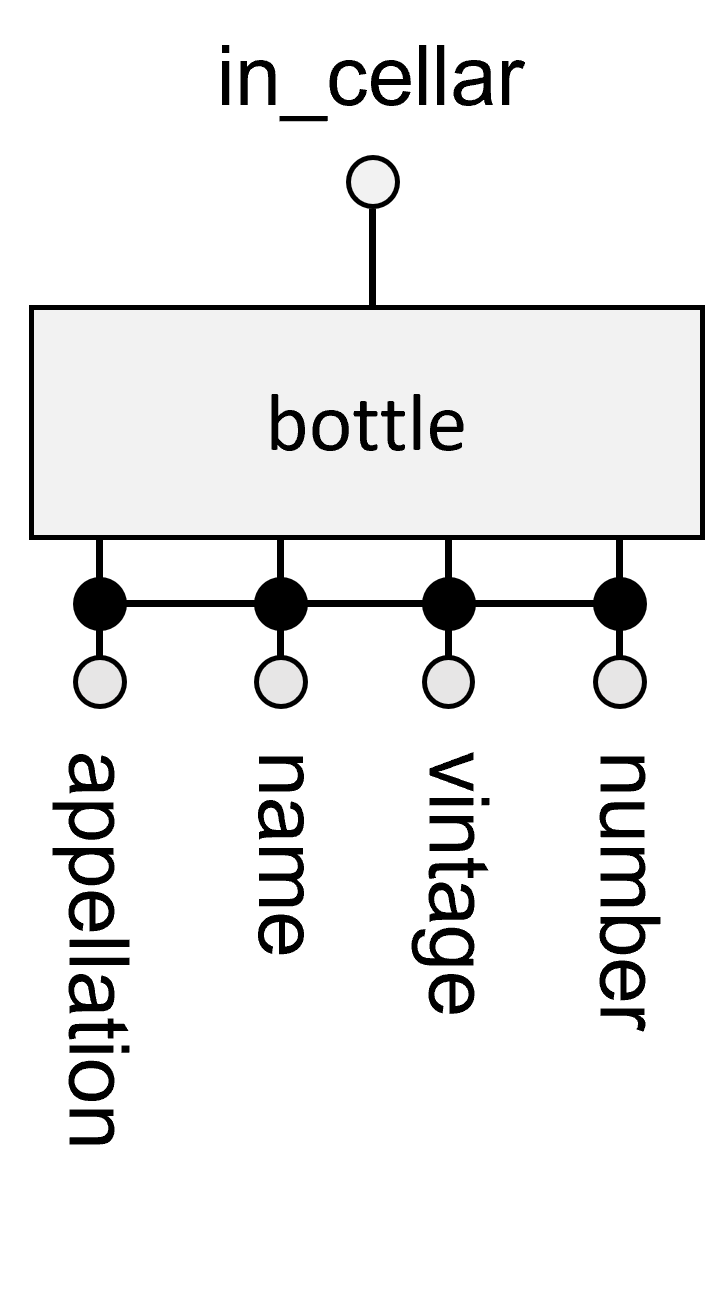
\includegraphics[width=1\textwidth]{t4/images/bottle_entity_3fk.png}
\end{columns}
\end{figure}	
\end{frame}

\begin{frame}[fragile]{Question 1 (a-d) Cont.}
Let's find the supporting text from the background information provided.\\ \vspace{5pt}

\begin{columns}[t]
	\column{0.76\textwidth}
	\begin{exampleblock}{Entity \textit{member} (Paragraph 1)}
		The organisation is big enough so that there could be several
		members with the same \underline{name}. A card with a unique \underline{number} is issued to \textbf{identify} each drinker. The \underline{contact address} of each member is also recorded for the mailing of announcements and calls for meetings.
	\end{exampleblock}
	\column{0.22\textwidth}
	\begin{figure}
		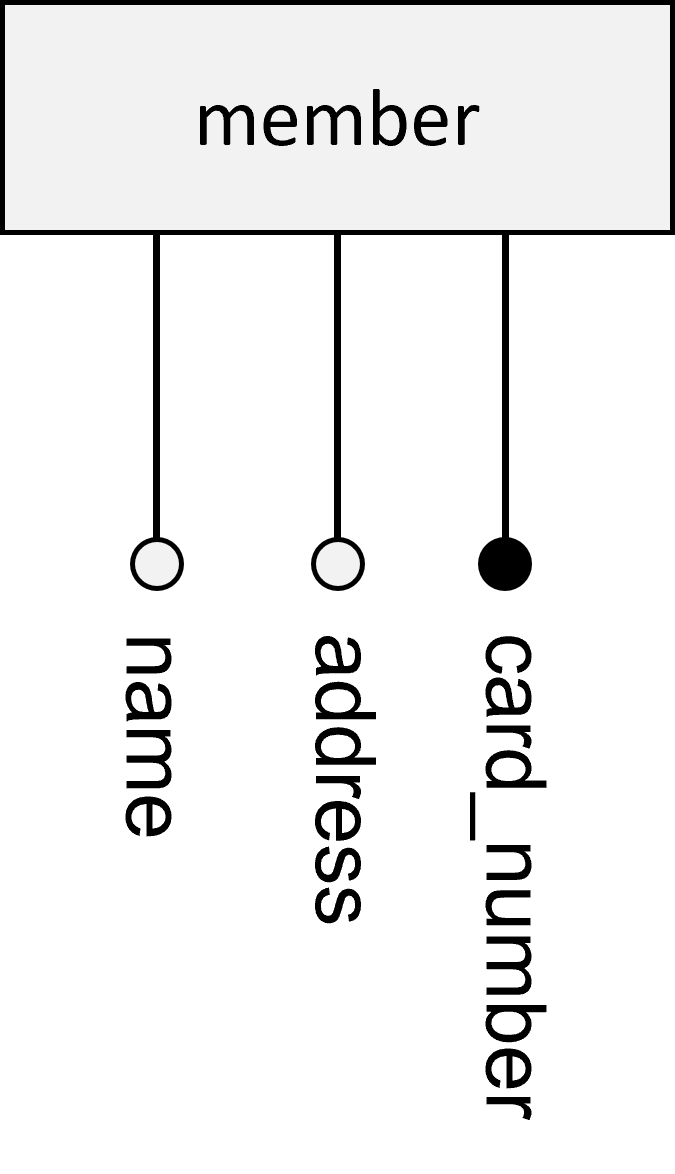
\includegraphics[width=1\textwidth]{t4/images/member_entity.png}
	\end{figure}
\end{columns}
\end{frame}

\begin{frame}[fragile]{Question 1 (a-d) Cont.}
\begin{columns}
	\column{0.68\textwidth}
	\begin{exampleblock}{Entity \textit{wine} (Paragraph 3)}
		Each wine is \textbf{identified} by its \underline{name} (Parade D'Amour), \underline{appellation} (Bordeaux) and \underline{vintage} (1990). Other information of interest about the wine is the \underline{degree of alcohol} (11.5), where and by whom it has been \underline{bottled} (Mis en Bouteille par Amblard-Larolphie Negociant-Eleveur a Saint Andrede Cubzac (Gironde) - France), the \underline{certification} of its appellation if available (Appellation Bordeaux Controlée), and the \underline{country} it comes from
		(produce of France).
	\end{exampleblock}
	\column{0.32\textwidth}
	\begin{figure}
		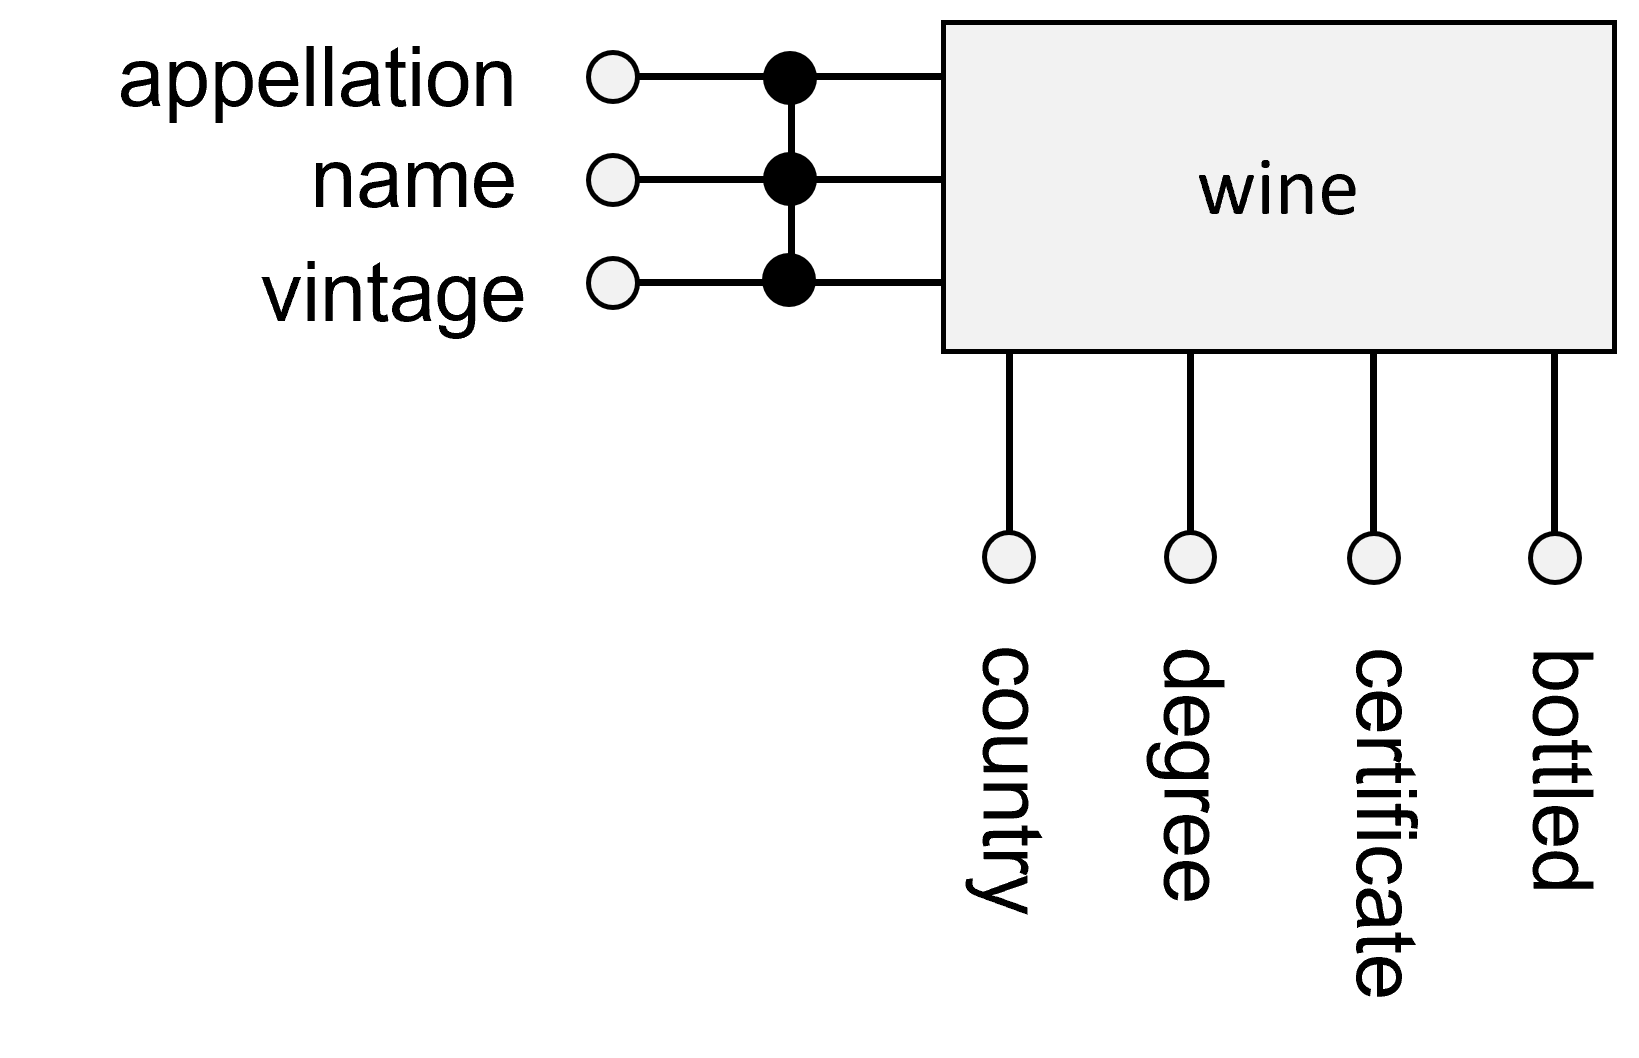
\includegraphics[width=1\textwidth, trim=0.9cm 0 0 0, clip]{t4/images/wine_entity.png}
	\end{figure}
\end{columns}
\end{frame}

\begin{frame}[fragile]{Question 1 (a-d) Cont.}
\begin{columns}
	\column{0.75\textwidth}
	\begin{exampleblock}{Entity \textit{bottle} (Paragraph 4)}
		\textbf{For each wine}, the bottles in the wine cellar of VINO are numbered. For instance, the cellar has 20 bottles \underline{numbered} 1 to 20 of a Semillon from 1996 named Rumbalara. ... The bottles are either available \underline{in the cellar} or they have been tasted and emptied.
	\end{exampleblock}
	\column{0.25\textwidth}
	\begin{figure}
		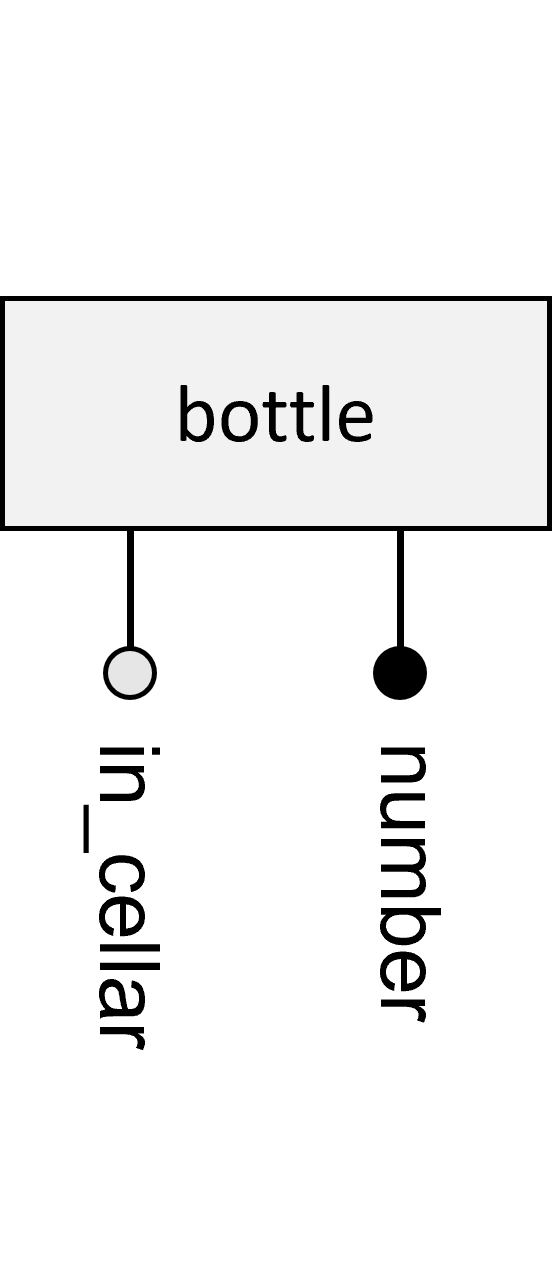
\includegraphics[width=0.8\textwidth, trim=0 0 0 0, clip]{t4/images/bottle_entity.png}
	\end{figure}
\end{columns}
\end{frame}

\begin{frame}[fragile]{Question 1 (a-d) Cont.}
\begin{exampleblock}{Relationship \textit{taste} (Paragraph 2)}
	At most once a week, VINO organises a tasting \textbf{session}. At each session, the attending members taste several	bottles. Each \textbf{member} records for each bottle his or her evaluation of the \textbf{quality} (very good, good, average, mediocre, bad, very bad) of each wine that she or he tastes. The evaluation may differ for the same wine from one drinker to another. Actual quality and therefore evaluation also varies from one to another \textbf{bottle} of a given wine. Every bottle that is opened during the tasting session is finished during that session.
\end{exampleblock}

\begin{figure}
	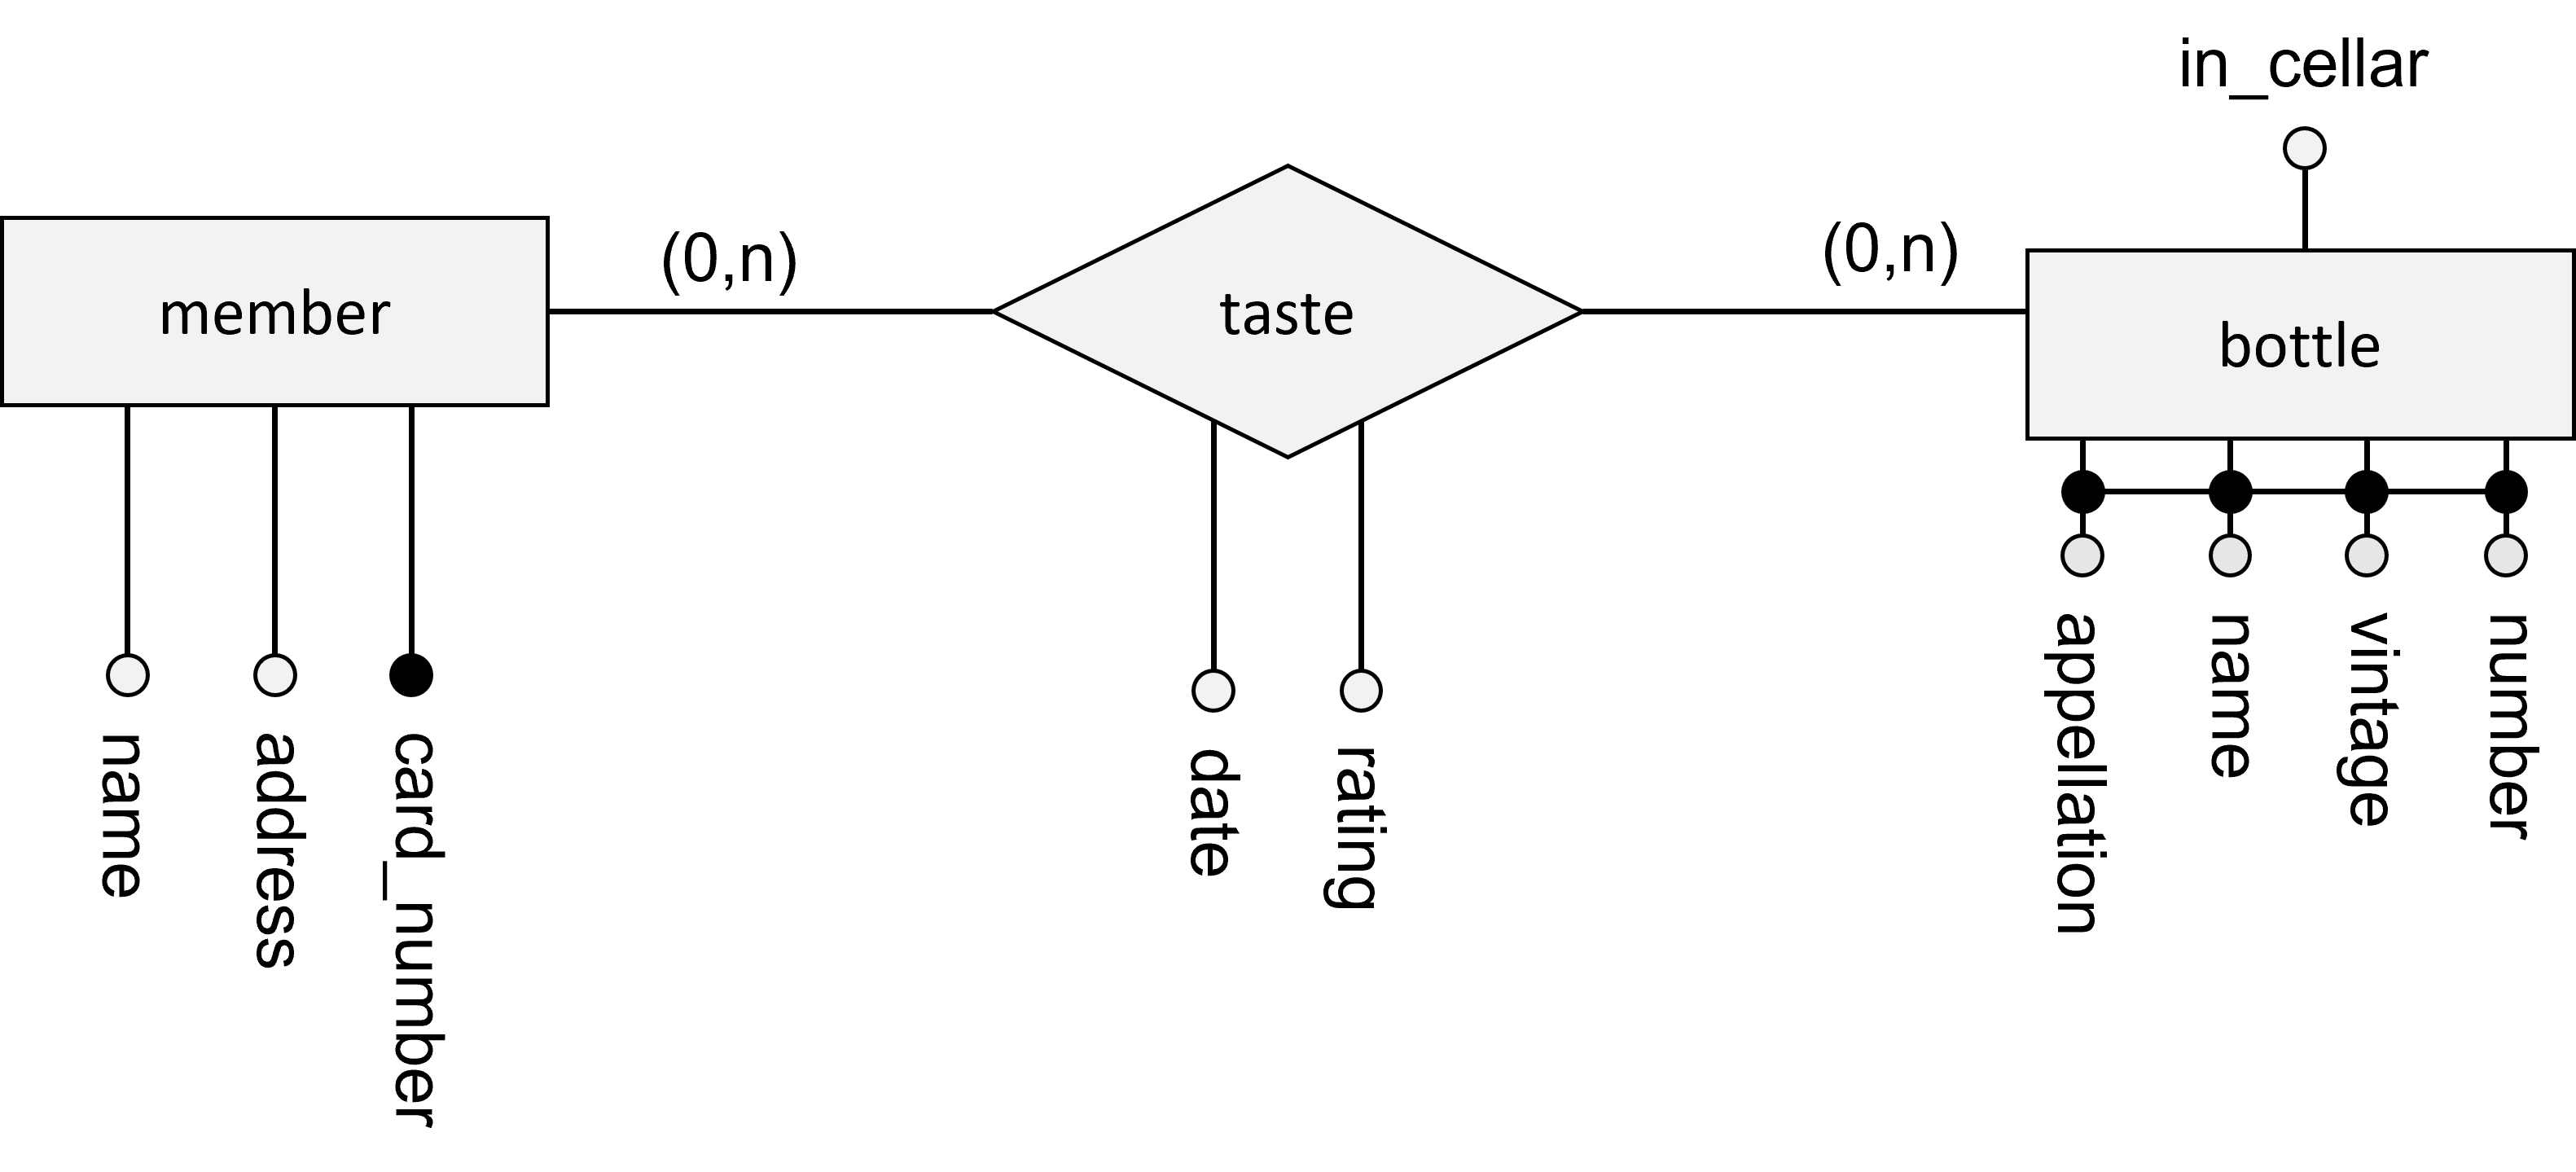
\includegraphics[width=0.8\textwidth]{t4/images/taste_relationship.png}
\end{figure}
\end{frame}

\begin{frame}[fragile]{Question 1 (a-d) Cont.}
\begin{columns}
	\column{0.64\textwidth}
	\begin{exampleblock}{Relationship \textit{contain} (Paragraph 4)}
		Generally, there are or have been several bottles of the same wine in the cellar...For documentation purposes VINO may also want to record wines for which it does not own bottles.
	\end{exampleblock}
	\column{0.36\textwidth}
	\begin{figure}
		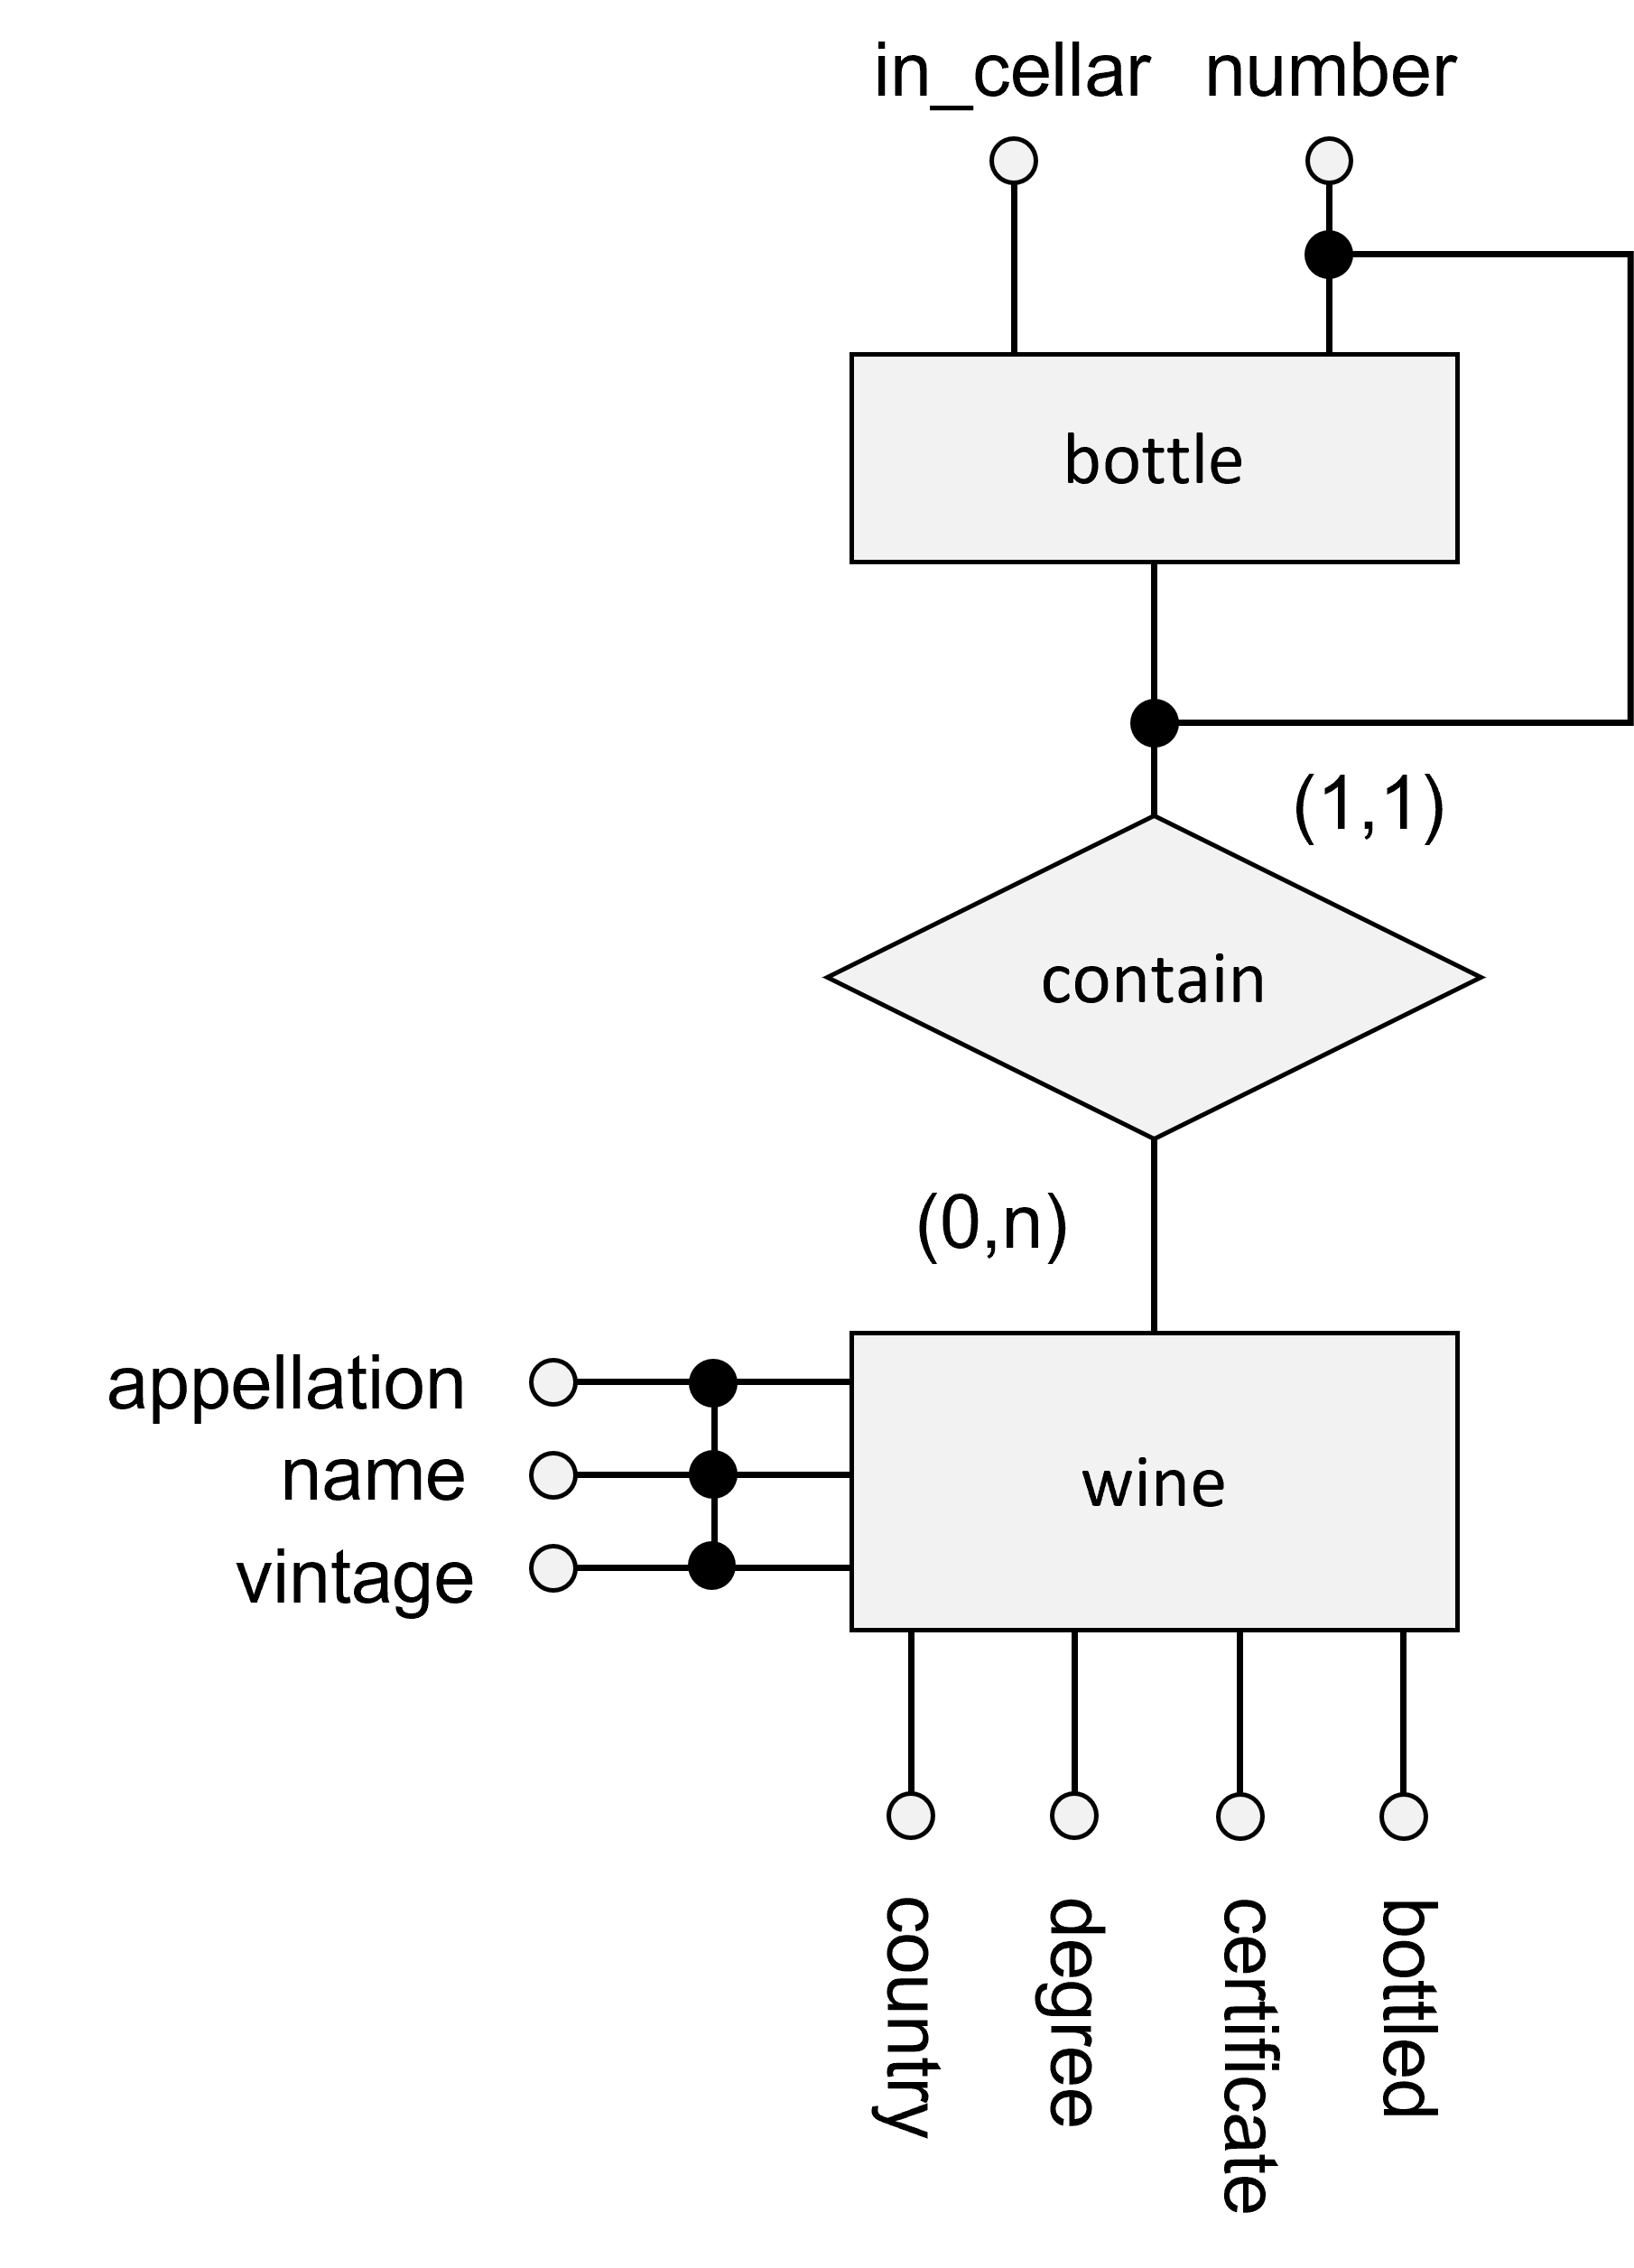
\includegraphics[width=0.8\textwidth, trim=1.1cm 0 0 0, clip]{t4/images/contain_relationship.png}
	\end{figure}
\end{columns}
\end{frame}

\begin{frame}[fragile]{Question 1 (e)}
For each entity set and each relationship set in which it participates, indicate the minimum and maximum participation constraints.\\ \vspace{10pt}
\textbf{Solution}: The relationship \textbf{taste} is an optional many-to-many relationship: both pairs of cardinality constraints are (0, n).\\ \vspace{5pt}
The relationship \textbf{contain} is a one-to-many relationship from wine to bottle. It is mandatory for the bottle entities and optional for the optional for the wine entities. The participation constraints for the entity set \textbf{wine} is (0, n). The participation constraints for the entity set \textbf{bottle} is (1, 1). It could not be otherwise since the entity set bottle is a weak entity (is weakly identified under the relationship set \textbf{contain} and the dominant entity set \textbf{wine}).
\end{frame}


\begin{frame}[fragile]{Question 1 (f)}
Draw the corresponding entity-relationship diagram with the key and participation constraints. Indicate in English the constraints that cannot be captured, if any.\\ \vspace{5pt}
\textbf{Solution}: There is no additional constraints.

\begin{figure}
	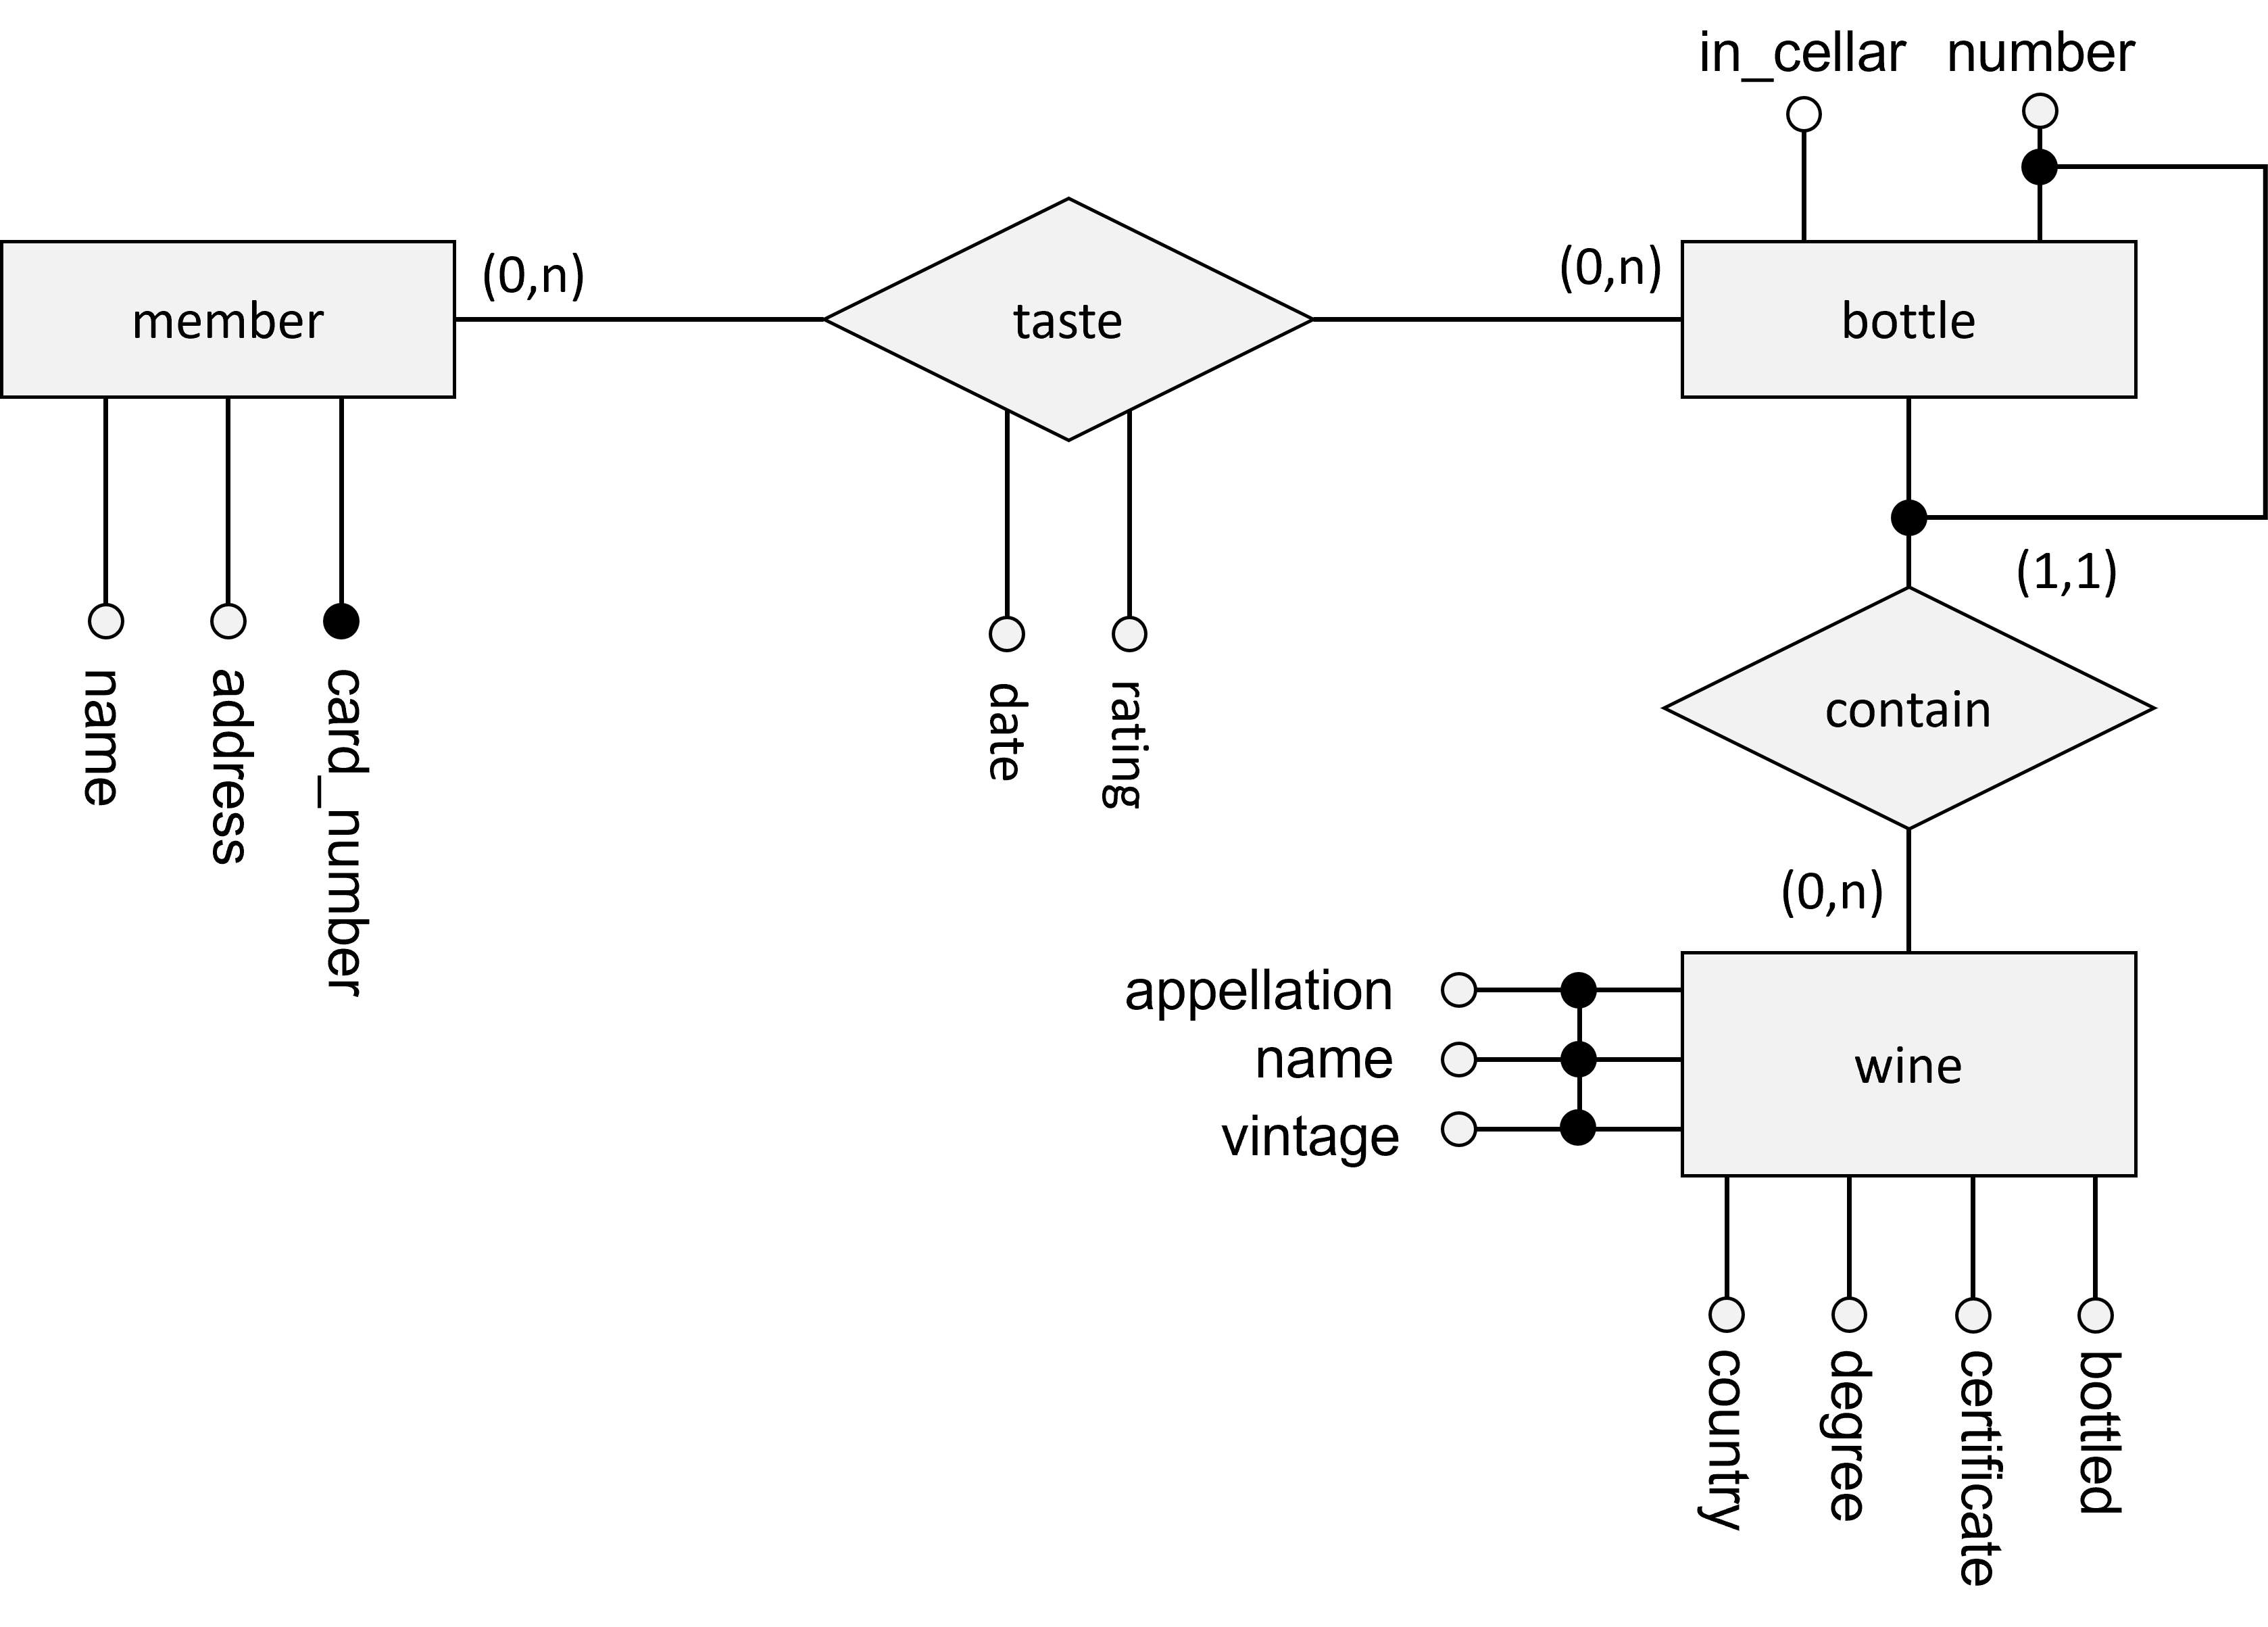
\includegraphics[width=0.75\textwidth, trim=0 0 0 0, clip]{t4/images/er_diagram.png}
\end{figure}
\end{frame}


\begin{frame}[fragile]{Question 2}
Translate your entity-relationship diagram into a relational schema. Give the SQL data description language (DDL) statements to create the schema. Declare the necessary integrity constraints. Indicate in English the constraints that cannot be captured, if any.
\end{frame}

\begin{frame}[fragile]{Question 2 Cont.}
\textbf{Solution}:
\begin{lstlisting}
CREATE TABLE IF NOT EXISTS members (
	name VARCHAR(20) NOT NULL,
	card_number NUMERIC PRIMARY KEY,
	address VARCHAR(50) NOT NULL
);

CREATE TABLE IF NOT EXISTS wines (
	name VARCHAR(20),
	vintage DATE,
	appellation VARCHAR(20),
	alcohol_degree NUMERIC NOT NULL,
	bottled VARCHAR(100) NOT NULL,
	certification VARCHAR(50),
	country VARCHAR(20) NOT NULL,
	PRIMARY KEY (name, vintage,appellation)
);

\end{lstlisting}
\end{frame}

\begin{frame}[fragile]{Question 2 Cont.}
\begin{lstlisting}[style=sql-small, firstnumber=17]
-- CONTINUED WITH THE LAST SLIDE
CREATE TABLE IF NOT EXISTS bottles (
	wine_name VARCHAR(20),
	vintage DATE,
	appellation VARCHAR(20),
	number INTEGER,
	PRIMARY KEY (number, wine_name, vintage, appellation),
	FOREIGN KEY (wine_name, vintage, appellation)
	REFERENCES wines (name, vintage, appellation)
);

CREATE TABLE IF NOT EXISTS taste (
	member NUMERIC(20),
	wine_name VARCHAR(20),
	vintage DATE,
	appellation VARCHAR(20),
	rating VARCHAR(9) NOT NULL,
	bottle_no INTEGER,
	date DATE NOT NULL,
	PRIMARY KEY (member, bottle_no, wine_name, vintage, appellation),
	FOREIGN KEY (member) REFERENCES members(card_number),
	FOREIGN KEY (bottle_no, wine_name, vintage,appellation) REFERENCES 
	bottles(number, wine_name, vintage, appellation)
);
\end{lstlisting}
\end{frame}

\begin{frame}[fragile]{Question 2 Cont.}
Logical diagram of tables created:

\begin{figure}
	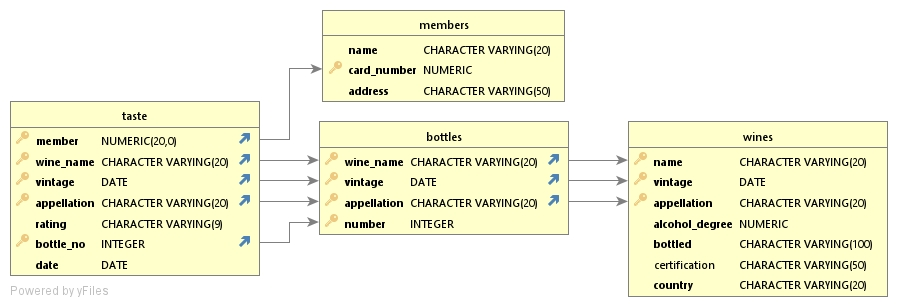
\includegraphics[width=0.85\textwidth, trim=0 0 0 0, clip]{t4/images/logical_diagram.jpg}
\end{figure}
\end{frame}
	
\begin{frame}{}
	\centering  
	For any further question, please feel free to email me:\vspace{10pt}
	
	huasong.meng@u.nus.edu \vspace{20pt}
	
	\begin{tcolorbox}
		\begin{center}
			\textcolor{red}{Copyright 2021 Mark H. Meng. All rights reserved.}
		\end{center}
	\end{tcolorbox}
\end{frame}